\documentclass[letterpaper,conference]{IEEEtran}

\usepackage{cite}
\usepackage{amsmath,amssymb,amsfonts}
\usepackage{graphicx}
\usepackage{booktabs}
\usepackage{array}
\usepackage{url}
\usepackage{balance}
\usepackage{placeins}

\graphicspath{{./figs/}{./}}
\newcommand{\seTwo}{\mathrm{SE}(2)}
\newcommand{\dchunk}{D_{\mathrm{chunk}}}
\newcommand{\dshape}{D_{\mathrm{shape}}}
\newcolumntype{L}[1]{>{\raggedright\arraybackslash}p{#1}}

\begin{document}

\title{SmolVLA for Language-Conditioned Driving:\\
Matched-Input and Closed-Loop Evaluation}

\author{
\IEEEauthorblockN{Sun Hong Jung}
\IEEEauthorblockA{\textit{Dept. of Electrical and} \\
\textit{Computer Engineering} \\
\textit{Sungkyunkwan University}\\
Suwon, Republic of Korea \\
tjsghd7867@g.skku.edu}
\and
\IEEEauthorblockN{Young Hoon Suh}
\IEEEauthorblockA{\textit{Dept. of Electrical and} \\
\textit{Computer Engineering} \\
\textit{Sungkyunkwan University}\\
Suwon, Republic of Korea \\
dudgns0407@g.skku.edu}
\and
\IEEEauthorblockN{Hyo Jin Park}
\IEEEauthorblockA{\textit{Dept. of Electrical and} \\
\textit{Computer Engineering} \\
\textit{Sungkyunkwan University}\\
Suwon, Republic of Korea \\
phyojin0511@g.skku.edu}
\and
\IEEEauthorblockN{Jae Wook Jeon$^*$}
\IEEEauthorblockA{\textit{Dept. of Electrical and} \\
\textit{Computer Engineering} \\
\textit{Sungkyunkwan University}\\
Suwon, Republic of Korea \\
jwjeon@skku.edu}
}

\maketitle

\begin{abstract}
Compact vision--language--action (VLA) models enable language-conditioned robot
control, but instruction use after adaptation to a vehicle embodiment remains
insufficiently characterized. We fine-tune SmolVLA for simulated closed-loop
control on 406 language-tagged demonstrations comprising 93,733 samples and 388
task strings. The policy maps front RGB, English instruction, speed, yaw rate,
and a constant legacy state slot to a 30-step incremental $\seTwo$ chunk. A
$2^3$ matched-input intervention varies the template, the tested
\emph{inner/outer}-to-\emph{innermost/outermost} replacement, and speed wording
across 20 fixed observations. Base wording gives 0.690-m median raw action-path
separation versus a 0.125-m lane-1 same-instruction reference. Template- and
speed-only changes retain 0.826 and 0.672~m, whereas the tested lane replacement
reduces separation to 0.093~m; the pattern persists after an offline bridge
transform. In 32 wall-clock rollouts balanced across two starts and both
instruction orders, Base different-instruction pairs yield 7.376-m median
trajectory separation versus a 0.177-m repeated-instruction reference. Every
post-15-m resampled point in all 16 Base rollouts is closer to the requested
lane, whereas all eight inner requests under the test wording are closer to the
outer reference. The results establish a measured language-to-motion path and
localize the observed loss to this tested replacement rather than sentence
novelty in general.
\end{abstract}

\begin{IEEEkeywords}
vision--language--action models, SmolVLA, language-conditioned driving, action chunking, closed-loop
evaluation, ROS~2
\end{IEEEkeywords}

\begin{figure*}[!t]
  \centering
  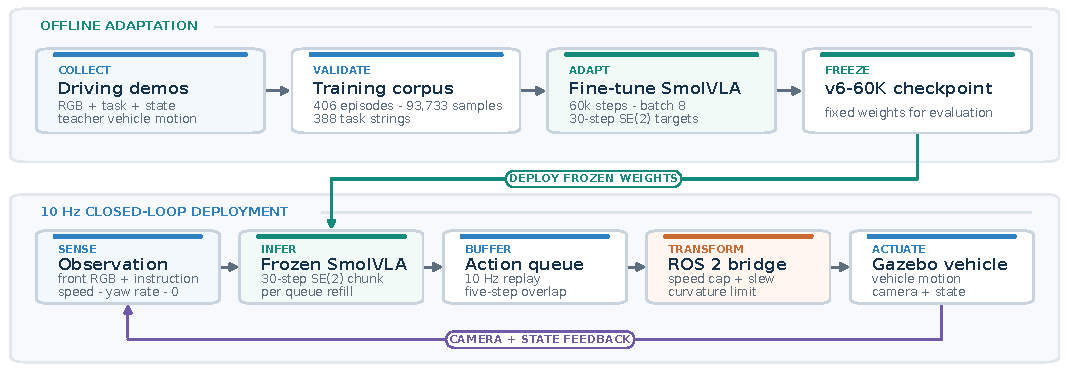
\includegraphics[trim=4.8bp 6.2bp 4.8bp 3.5bp,clip,width=\textwidth]{fig1_language_pipeline.pdf}
  \caption{Training and deployment pipeline. Frozen SmolVLA maps RGB, language,
  and state to 30-step $\seTwo$ chunks replayed at 10~Hz in ROS~2--Gazebo.}
  \label{fig:pipeline}
  \vspace{-7pt}
\end{figure*}

\section{Introduction}
Vision--language--action models promise a common interface between natural
language, visual perception, and continuous robot control. OpenVLA showed that
an open pretrained VLA can be adapted to multiple manipulation platforms and
tasks~\cite{openvla}, while SmolVLA reduced the policy scale to roughly 450M
parameters and retained chunked continuous actions~\cite{smolvla}. The smaller
model is attractive for robot and vehicle prototypes, but adapting it to a new
embodiment raises a basic empirical question: does the fine-tuned policy use the
instruction to choose motion, or does it mostly reproduce the visually likely
route?

Vehicle driving makes that distinction observable. Two lane instructions can
share the same initial camera view and vehicle state yet require different
future paths. A policy that ignores language may still drive smoothly, so
completion or lane keeping alone cannot establish language conditioning.
Conversely, a difference between two stochastic policy samples is not by itself
evidence that changing the instruction caused the difference. Evaluation must
therefore hold the visual and state observations fixed, compare the resulting
action chunks against a disjoint-seed same-instruction reference, and determine
whether the separation persists after the actions enter a closed loop.

We study a SmolVLA checkpoint fine-tuned on language-tagged demonstrations for
a simulated vehicle-like platform. The policy receives one front image, an
English sentence, speed, yaw rate, and a constant legacy state slot, and
predicts 30 incremental ego-motion actions. It is deployed through a ROS~2 bridge in
Gazebo, where the bridge deterministically maps the checkpoint output to motion
commands. Rather than claim broad natural-language understanding, we compare
Base wording assembled from observed components with a symmetric test wording
pair assembled from phrase-bank components absent from the vehicle fine-tuning
inventory. None of the 16 complete evaluation sentences occurs verbatim in the
recovered final task inventory. We vary the three wording components
factorially to identify which tested change is associated with lost lane response.

The contributions are threefold:
\begin{enumerate}
    \item a compact-VLA adaptation pipeline for language-conditioned vehicle
    control, from validated demonstrations to 30-step incremental $\seTwo$
    chunks and ROS~2--Gazebo execution;
    \item a matched-observation $2^3$ intervention that separates template,
    the tested \emph{inner/outer}-to-\emph{innermost/outermost} replacement,
    and speed-term effects and checks both raw paths and an offline
    bridge-transformed sensitivity path; and
    \item 32 balanced closed-loop rollouts showing that the baseline language
    distinction survives vehicle execution, together with the closed-loop
    failure observed for that tested replacement.
\end{enumerate}

\section{Related Work}
OpenVLA established open downstream VLA adaptation, while SmolVLA combines a
compact backbone with flow-matching action chunks~\cite{openvla,smolvla}.
ROS2SmolVLA integrates SmolVLA with an industrial manipulator through
ROS~2~\cite{ros2smolvla}; our embodiment and evaluation instead concern planar
vehicle control and the measured effect of driving instructions.

Within our laboratory's scaled-vehicle lineage, Oh \emph{et al.} developed a
competition-based autonomous-driving education framework~\cite{oh2026education},
and Hong \emph{et al.} compared rule-based and learned end-to-end vehicle
control~\cite{hong2025datadriven}. Suh \emph{et al.} evaluated a modular
detector--VLM driving stack~\cite{suh2025modularvla} and later a latency-aware
slow/fast safety-arbitration architecture~\cite{suh2026lasa}. These works
establish the platform, learning, and VLA lineage for the present study. We
reuse that lineage's simulated track and its fixed inner/outer lane identities,
but each episode instruction here names a lane, a speed term, and often a
destination or stop target rather than a single lane-change command.

SimLingo studies language-aligned closed-loop driving, and OpenDriveVLA predicts
trajectories from perception, state, and driver commands~\cite{simlingo,opendrivevla}.
LinkVLA directly trains language--action alignment~\cite{linkvla}, while
ICR-Drive isolates instruction effects under controlled text
changes~\cite{icrdrive}. Manipulation benchmarks report the same class of
failure: counterfactual instruction assignment under visually plausible layouts
exposes vision shortcuts~\cite{liberocf}, and synonym-level paraphrase alone
degrades task success~\cite{liberopara}. We therefore do not claim the failure
mode itself as new. In contrast to these evaluations, we freeze the exact
RGB/state input for a factorized action-chunk intervention on a vehicle policy
and then test whether the measured distinction persists through a
ROS~2--Gazebo closed-loop executor.

\section{Methodology}
Figure~\ref{fig:pipeline} summarizes the full system, and
Table~\ref{tab:configuration} lists the training and deployment configuration.
The learned component is the fine-tuned SmolVLA policy; the same frozen
checkpoint is used in every reported evaluation.

\subsection{Demonstration Corpus}
A teacher controller generated ring-driving motion while an episode-level
English instruction specified lane and speed, often together with a landmark
destination or stop task. Each
raw episode contained a front-camera stream, the language label, vehicle state,
teacher control, and global pose at 30~Hz. Validation rejected incomplete or
geometrically invalid episodes, and retained records were resampled into a
10-Hz LeRobot-style representation. The final v6 LeRobot metadata records 406
episodes, 93,733 action rows, and 388 distinct task strings, which compose lane,
speed, and destination slots over paraphrased surface forms across six named
track targets and a lap form. That composition is a premise of the later test:
lane is one slot among three, so a lane-dependent response cannot come from
matching two fixed strings, and the template and speed slots supply the other
two wording factors. We recovered the
complete task inventory from the training artifact and stored its sorted hash
with the evaluation records.

The checkpoint's three-value state is
\begin{equation}
\mathbf{s}_t=[v_t,\dot{\psi}_t,0],
\label{eq:state}
\end{equation}
where $v_t$ and $\dot{\psi}_t$ denote vehicle speed and yaw rate. The third,
legacy state slot is identically zero in all 93,733 training rows and is forced
to zero at evaluation; it is not treated as a measured steering signal. Global
position and map coordinates are excluded from policy input. A training target
is the ego-frame displacement over one 0.1-s step,
$\mathbf{a}_i=[\Delta x_i,\Delta y_i,\Delta\psi_i]$. Language is therefore the
only direct specification of which lane the policy should follow when the
initial visual and state observations are identical.

\subsection{Policy and Fine-Tuning}
Starting from the compact SmolVLA release, we fine-tune a policy that predicts
\begin{equation}
\mathbf{A}_t=\pi_\theta(I_t,\ell,\mathbf{s}_t),\qquad
\mathbf{A}_t\in\mathbb{R}^{30\times3},
\label{eq:policy}
\end{equation}
where $I_t$ is the front RGB image and $\ell$ is the English task. Training
runs for 60,000 optimization steps with batch size 8, learning rate $10^{-4}$,
automatic mixed precision, seed 1000, and no image augmentation. This
corresponds to approximately 5.12 passes over the 93,733-row corpus. The
resulting v6-60K checkpoint is frozen for all experiments.

The checkpoint retains SmolVLA's SmolVLM2-500M-Video-Instruct backbone,
cross-attention action conditioning, and ten flow-matching denoising steps. We
update the full policy with AdamW, a 1,000-step warmup, and cosine decay; all
settings are held fixed across language conditions.

The predicted increments are composed into an ego-frame path for analysis:
\begin{equation}
\mathbf{p}_0=\mathbf{0},\qquad
\mathbf{p}_{i+1}=\mathbf{p}_i\oplus\mathbf{a}_i,\quad i=0,\ldots,29,
\label{eq:compose}
\end{equation}
where $\oplus$ applies the translation after rotating it by accumulated yaw.
This is a diagnostic path composed from the \emph{raw} policy output, including
$\Delta y$; it is not a simulated vehicle trajectory. Deployed replay uses
$\Delta x$ and $\Delta\psi$, as specified below, and closed-loop evaluation
measures the resulting vehicle motion.

\begin{table}[!ht]
\caption{Training and Deployment Configuration}
\label{tab:configuration}
\centering
\footnotesize
\setlength{\tabcolsep}{3.0pt}
\begin{tabular}{@{}L{0.28\columnwidth}L{0.64\columnwidth}@{}}
\toprule
Item & Configuration \\
\midrule
Policy & SmolVLA, approx. 450M parameters; frozen v6-60K checkpoint \\
Corpus & 406 episodes; 93,733 rows at 10~Hz; 388 task strings \\
Observation & Front RGB; English task; speed, yaw rate, constant-zero legacy slot \\
Action & $30\times[\Delta x,\Delta y,\Delta\psi]$ at 0.1-s intervals \\
Fine-tuning & 60K steps; batch 8; LR $10^{-4}$; AMP; seed 1000; no image augmentation \\
Queue & 10~Hz; five-step overlap; refill at 30\% remaining; direct replay \\
Command limits & 2.25-m/s speed; 0.08-m/s/tick slew; 0.239-m$^{-1}$ curvature \\
Evaluation & One ring; two matched starts; 30-s wall-clock runs; policy seed 0 \\
\bottomrule
\end{tabular}
\end{table}

\subsection{ROS~2--Gazebo Deployment}
The ROS~2 deployment~\cite{ros2} sends the image, state, and latched task to a
policy server and receives a 30-step action chunk. A bridge maintains a queue
with five-step overlap and requests a new chunk when 30\% remains. At each
10-Hz tick, direct replay obtains the raw speed and curvature,
\begin{equation}
v_i^{0}=\frac{\Delta x_i}{0.1},\qquad
\kappa_i^{0}=\frac{\Delta\psi_i}{\Delta x_i}\quad(|\Delta x_i|>10^{-4}\ \mathrm{m}),
\label{eq:replay}
\end{equation}
then caps speed at 2.25~m/s, limits its per-tick change to 0.08~m/s, clips
$\kappa_i^0$ to $\pm0.239$~m$^{-1}$, and publishes
$\omega_i=\kappa_i v_i$. When $|\Delta x_i|\le10^{-4}$~m, the raw yaw rate is
retained instead. The lateral prediction $\Delta y_i$ is not sent to the
executor. Gazebo closes the camera and state loop around a vehicle-shaped model
whose body motion is implemented by a differential-drive plugin~\cite{gazebo}.
Front steering joints visualize the corresponding curvature but do not define
the body dynamics. No map, goal vector, or global pose is sent to the policy.

The server senses one front image, takes its camera key from the checkpoint,
and recovers the actual three-value state width from the saved normalizer.
Inherited unused camera slots and the base configuration's placeholder
six-value state shape are ignored.

For evaluation, the simulator is paused after each matched commanded-pose
reset, the instruction is published, and execution begins only after the first action
chunk arrives. This prefill protocol prevents startup delay from being counted
as a controller watchdog failure; it does not change the predicted actions or
the subsequent closed-loop control. A rollout is accepted only if the
commanded position is verified within 5~cm, the trajectory contains at least
five retained points, and both watchdog activations and action underruns remain
zero.

\subsection{Evaluation Protocol}
\subsubsection{Matched-observation action test}
We sample 20 validated lane-counterfactual groups from three collection
sessions in the v6 training lineage and select 10-Hz row index 5 (nominally
0.5~s after the common start). For each group, the exact same RGB array and state vector are supplied
to both sides; only the instruction differs. A $2^3$ design changes three
binary wording components: template $T$ (``Start driving''/``Roam the track''),
lane replacement $L$ (``inner, outer''/``innermost, outermost''), and speed term $S$
(``normal''/``regular''). This gives Base, $T$, $L$, $S$, $T{+}L$, $T{+}S$,
$L{+}S$, and $T{+}L{+}S$ cells with unchanged lane semantics.

None of the 16 complete evaluation sentences appears verbatim in the recovered
388-task training inventory. The Base components occur in that inventory,
whereas all alternate $T$, $L$, and $S$ components occur zero times and belong
to a phrase bank committed before v6 training. Thus the design localizes the
response within this fixed wording set; the visual observations themselves are
not held out.

SmolVLA sampling is stochastic. We average four predicted chunks for each
instruction using seeds 0--3. For context, the same image, state, and lane-1
sentence are sampled again with disjoint seeds 4--7. This is an asymmetric
lane-1 same-instruction reference, not an upper bound on stochastic variation
for both instructions. Let
$P_{xy}(\ell)=\{\mathbf{p}_{i,xy}(\ell)\}_{i=1}^{30}$ contain the translation
components of the raw composed poses from~\eqref{eq:compose}. Instruction
separation is
\begin{equation}
\dchunk(\ell_1,\ell_2)=
\sqrt{\frac{1}{30}\sum_{i=1}^{30}
\left\|\mathbf{p}_{i,xy}(\ell_1)-\mathbf{p}_{i,xy}(\ell_2)\right\|_2^2}.
\label{eq:dchunk}
\end{equation}
For each observation we also report $R=\dchunk/D_{\mathrm{ref},1}$, where
$D_{\mathrm{ref},1}$ applies~\eqref{eq:dchunk} to the disjoint-seed lane-1
chunks; $R>1$ exceeds this scoped same-instruction reference.
Factor effects are saturated contrasts of
$\log_2(\dchunk/1\,\mathrm{m})$, computed within each observation and
summarized with a 50,000-resample paired bootstrap. The
intervals are exploratory pointwise intervals over this fixed sample.

The saved four-seed mean chunks also support a zero-initial-command
bridge-transform sensitivity check. Although the observation speed spans
0.562--2.181~m/s, this diagnostic initializes the
\emph{previous commanded} speed to zero, drops $\Delta y$, applies the recorded
speed cap and slew together with the source-defined curvature clip
in~\eqref{eq:replay}, integrates the resulting unicycle commands, and
recomputes separation. It does not emulate queue refill, splicing, or Gazebo;
those effects are evaluated only by the closed-loop runs.

\subsubsection{Paired closed-loop test}
The closed loop evaluates only the two factorial endpoints, Base and
$T{+}L{+}S$; localization of the individual factors is action-level only. We
use inner- and outer-lane starts at the same longitudinal track index. For each
wording regime and start, one invocation uses inner then outer (AB) and a
second uses outer then inner (BA). Each invocation records a same-instruction
pair $(A,A)$ followed by a different-instruction pair $(A,B)$. Thus both
same-inner and same-outer references and both instruction orders are observed at
each start: $2$ regimes $\times2$ starts $\times2$ orders $\times4$ physical
rollouts gives 32 rollouts. Each lasts 30~s wall clock with policy seed 0.

The spatially thinned trajectories are truncated to their common traveled
length, and their discrete Fr\'{e}chet distance is reported as
$\dshape$. This metric measures path separation while respecting trajectory
order. The shared prefix is the traveled distance before the resampled paths
first differ by more than 0.30~m. Both are behavioral differentiation metrics:
they do not by themselves establish correct lane occupancy or safe driving.

To add a directional check, we discard the first 15~m of each trajectory so
the common start and lane transition do not dominate the result. For every
remaining point $\mathbf{x}$, we compute its Euclidean distance to the two
configured lane-center polylines, $R_1$ and $R_2$. For an instruction requesting
lane $\ell$, we report the per-run median and 95th percentile of
\begin{equation}
d_\ell(\mathbf{x})=\min_{\mathbf{r}\in R_\ell}
\|\mathbf{x}-\mathbf{r}\|_2,
\label{eq:lane_distance}
\end{equation}
where the implementation projects onto line segments rather than only sampled
vertices. We also report the fraction of analyzed points for which
$d_\ell(\mathbf{x})<d_{3-\ell}(\mathbf{x})$. This is a centerline-relative route
check, not a lane-boundary or collision-safety metric.

\subsubsection{Reproducibility and validity controls}
Independent SHA-256 checks verify that the closed-loop and offline evaluations
use the same checkpoint; the full digest is retained in the checkpoint
manifest. The recovered training inventory and hash, 20 observation
identifiers and state vectors, raw mean chunks, per-seed protocol, full closed-loop XY
traces, exact strings, reset coordinates, unique rollout IDs, applied bridge
contract, latency, watchdog count, and underrun fraction are retained in the
project evaluation records. Plot and table values are regenerated without
invoking the policy or simulator. No empty-language control is reported because
an empty task disarms the deployed bridge.

\section{Results}
\subsection{Instruction Conditioning of Action Chunks}
Figure~\ref{fig:chunks} plots all 20 observation-level
language/reference ratios in each wording cell, while Table~\ref{tab:chunks}
reports exact summaries. Without $L$, median $R$ is 5.14--6.15 and every cell
exceeds the reference in 20/20 observations. With the tested replacement of
\emph{inner/outer} by \emph{innermost/outermost} ($L$), median $R$ falls to
0.42--0.52 with only 0--1/20 exceedances; raw $\dchunk$ similarly separates
into 0.672--0.826~m without $L$ and 0.062--0.093~m with $L$.

\begin{figure}[!ht]
  \centering
  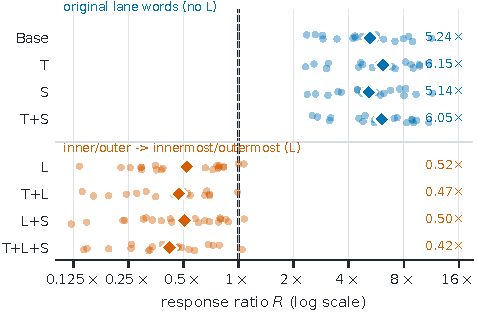
\includegraphics[width=0.99\columnwidth]{fig3_wording_factorial.pdf}
  \caption{Raw response ratio $R$ across the eight wording cells. Small points
  are 20 matched observations and diamonds are medians; $R=1$ (dashed) equals
  the disjoint-seed lane-1 same-instruction reference. $T$, $L$, and $S$
  denote template, the tested lane replacement, and speed terms.}
  \label{fig:chunks}
\end{figure}

\begin{table}[!ht]
\caption{$2^3$ Matched-Observation Raw Action Separation}
\label{tab:chunks}
\centering
\footnotesize
\setlength{\tabcolsep}{3.0pt}
\begin{tabular}{@{}lcccc@{}}
\toprule
Cell$^a$ & \shortstack{$\dchunk$\\Lang. (m)} & \shortstack{Lane-1\\ref. (m)} & \shortstack{Median\\ratio$^b$} & \shortstack{Above\\ref.} \\
\midrule
Base & 0.690 & 0.125 & 5.24 & 20/20 \\
$T$ & 0.826 & 0.123 & 6.15 & 20/20 \\
$S$ & 0.672 & 0.121 & 5.14 & 20/20 \\
$T{+}S$ & 0.823 & 0.123 & 6.05 & 20/20 \\
$L$ & 0.093 & 0.250 & 0.52 & 1/20 \\
$T{+}L$ & 0.062 & 0.205 & 0.47 & 0/20 \\
$L{+}S$ & 0.090 & 0.218 & 0.50 & 1/20 \\
$T{+}L{+}S$ & 0.063 & 0.220 & 0.42 & 1/20 \\
\bottomrule
\multicolumn{5}{@{}l}{\scriptsize $^aT$: template; $L$: tested lane replacement; $S$: speed term.}\\[-1pt]
\multicolumn{5}{@{}l}{\scriptsize $^b$Median of per-observation language/reference ratios.}
\end{tabular}
\end{table}

Separately, the raw-$\dchunk$ factorial contrast gives an $L$ effect of
$-3.118$ on $\log_2(\dchunk/1\,\mathrm{m})$, with a
paired-bootstrap 95\% interval of $[-3.469,-2.797]$, corresponding to a
factorial geometric-mean multiplier of 0.115. On the multiplier scale, the
$T$ main effect and $T{\times}L$ interaction are 0.916 $[0.852,0.984]$ and
0.828 $[0.769,0.890]$, respectively. The log-scale intervals for $S$ and the
remaining interactions span zero.
Thus $L$ is the dominant, but not exclusive, negative factor in this fixed
offline wording intervention.

The zero-initial-command bridge-transform check gives the same dominant factor:
$L=-3.339$ $[-3.704,-3.009]$, a geometric-mean multiplier of 0.099. Its Base
and $T{+}L{+}S$ medians are respectively 0.221 versus 0.031~m and 0.016 versus
0.037~m against their lane-1 references. All eight cells retain the same
above/below-reference median classification under raw and transformed paths.

\begin{figure*}[!t]
  \centering
  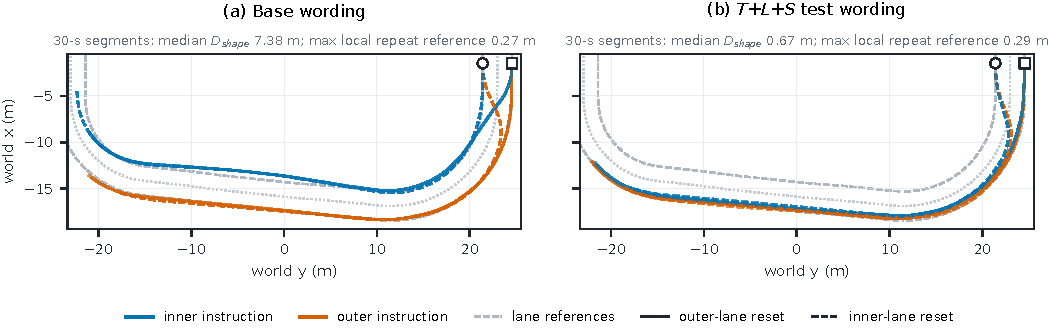
\includegraphics[width=0.985\textwidth]{fig2_closed_loop_language.pdf}
  \caption{Thirty-second wall-clock closed-loop segments from matched resets.
  Colors denote requested lanes and line styles denote reset lanes; gray curves
  are lane references. Base wording selects both routes, whereas the
  $T{+}L{+}S$ test wording collapses toward the outer route.}
  \label{fig:closedloop}
\end{figure*}

\subsection{Closed-Loop Language Response}
The closed-loop results in Fig.~\ref{fig:closedloop} and
Table~\ref{tab:closedloop} provide a directional complement to the action-level
test. Base wording
produces $\dshape=7.376$~m across the four different-instruction pairs, compared
with a 0.177-m median over the four same-instruction pairs. All four differences
exceed the local repeated-instruction reference for their own reset, defined as the larger of the
same-inner and same-outer values. The result holds at both starts and in both
AB and BA orders; the first $>0.30$-m divergence occurs after a median 2.5~m.

\begin{table}[!ht]
\caption{Paired Closed-Loop Trajectory Separation}
\label{tab:closedloop}
\centering
\footnotesize
\setlength{\tabcolsep}{1.6pt}
\begin{tabular}{@{}lcccc@{}}
\toprule
Wording & \shortstack{Different $\dshape$\\median [range] (m)} & \shortstack{Same $\dshape$\\median [range] (m)} & \shortstack{Above local\\ref.} & \shortstack{Shared\\prefix (m)} \\
\midrule
Base & 7.376 [6.740, 7.860] & 0.177 [0.167, 0.265] & 4/4 & 2.5 \\
$T{+}L{+}S$ & 0.666 [0.569, 0.889] & 0.243 [0.173, 0.292] & 4/4 & 10.3 \\
\bottomrule
\end{tabular}
\end{table}

Table~\ref{tab:adherence} checks whether the separation has the requested
direction. After 15~m, all sampled points in all 16 Base-wording rollouts
are closer to the requested reference. Across eight rollouts per target, the
median of run-level median offsets is 0.339~m for inner and 0.086~m for outer;
the corresponding median run-level 95th percentiles are 0.728 and 0.277~m.

\begin{table}[!ht]
\caption{Run-Level Centerline Adherence After 15~m (Eight Runs/Target)}
\label{tab:adherence}
\centering
\footnotesize
\setlength{\tabcolsep}{3.1pt}
\begin{tabular}{@{}llccc@{}}
\toprule
Wording & Request & \shortstack{Median of\\run medians (m)} & \shortstack{Median of\\run P95s (m)} & \shortstack{Median run\\fraction (\%)} \\
\midrule
Base & Inner & 0.339 & 0.728 & 100 \\
Base & Outer & 0.086 & 0.277 & 100 \\
$T{+}L{+}S$ & Inner & 2.779 & 3.019 & 0 \\
$T{+}L{+}S$ & Outer & 0.159 & 0.303 & 100 \\
\bottomrule
\end{tabular}
\end{table}

For $T{+}L{+}S$ wording, the different-instruction median is 0.666~m versus a
0.243-m same-instruction median, and the shared prefix increases to 10.3~m.
Although all four differences exceed their local references, separation alone is
not correctness. Every 0.2-m-resampled post-15-m point from all eight
inner-request rollouts is closer to the \emph{outer} reference, whereas the
corresponding points in all eight outer-request rollouts are closer to the outer
reference. The same 0\%/100\% target split holds for 10-, 15-,
and 20-m cutoffs and from both reset lanes. Base stay and change maneuvers
each have a median closer-to-target fraction of 1.0; $T{+}L{+}S$ gives 0.5
for each because behavior depends on the outer-lane bias, not the requested
maneuver.

All 32 rollouts satisfy the logged execution contract: watchdog hits and action
underrun are zero, steering-state source is constant zero, and the applied speed
cap is 2.25~m/s. First-chunk prefill is 0.239--0.299~s and the bridge's running
mean request round-trip time is 242.1--251.4~ms. The trajectories cover 52.74--58.98~m in
30~s wall clock, approximately 0.37--0.42 of the 141.97-m nominal centerline
length rather than a full lap.

\subsection{Discussion of Scope and Differentiation}
The combined tests provide evidence at two interfaces. At the policy
interface, Base inner/outer wording changes the 30-step motion prediction
under identical perception and state. At the embodiment interface, the same
distinction remains large after repeated perception, queue refill, and vehicle
dynamics close the loop. Together, these results demonstrate the feasibility
of language-conditioned control with the fine-tuned compact VLA in the
evaluated simulator; no comparison against alternative policies is implied.

The result for the test wording is pair-specific: within this fixed factorial
set, only combinations retaining \emph{inner/outer} produce a robust
lane-dependent action change. The tested \emph{innermost/outermost} replacement
does not establish a general failure on unseen lane terms. Since none of the 16
complete evaluation sentences occurs in the task inventory, exact-string
novelty is insufficient evidence of language generalization. A vehicle VLA
evaluation should factor wording components and measure each response against a
clearly scoped same-instruction reference.

This work does not introduce a new VLA architecture or action-chunk executor.
Its contribution is an embodiment and evaluation methodology: an action-level
matched-input test prevents visually plausible driving from being mistaken for
language use, while the paired closed-loop test determines whether the measured
conditioning is large enough to affect the simulated vehicle trajectory.

\subsection{Threats to Validity}
The experiments use one simulator track, two matched starts, two lane intents,
English instructions, one vehicle snapshot, and one fine-tuned checkpoint. Speed and
destination slots are held semantically fixed, so no claim is made about their
conditioning. The
32 closed-loop trials are sequential runs with policy seed 0, not independent
training or simulator seeds; no significance claim is made. AB/BA balances
instruction order, but SAME always precedes DIFFERENT within an invocation.
Reset position is verified within 5~cm; yaw is logged but not an acceptance
tolerance. The 20 matched observations come from three collection sessions in
the training lineage, so they test conditioning interventions on fixed images,
not visual or scene generalization. The symmetric test wording pair was
selected after an exploratory offline probe; its factorial and closed-loop
results characterize a known failure and are not an unbiased estimate of
paraphrase success. The pointwise bootstrap treats the 20 matched observations
as its resampling units; it does not model collection-session clustering,
checkpoint-training uncertainty, or additional policy-sampling uncertainty.
Rollouts use a 30-s wall-clock horizon while the control timer follows ROS/Gazebo
simulation time; simulator real-time factor and elapsed simulation time were not
stored. Consequently, the reported distance and wall time are not a standardized
simulation-time speed benchmark.

An unadapted SmolVLA checkpoint has no compatible vehicle action normalizer, so
we do not report a numerical pretrained-policy baseline and do not claim that
fine-tuning improves a pre-existing driving score. Likewise, $\dchunk$ and
$\dshape$ measure separation rather than route correctness, lane-boundary
clearance, passenger comfort, or safety. No traffic, obstacles, weather,
sensor faults, real vehicle, or functional-safety property is evaluated.
The vehicle-shaped simulator uses differential-drive body dynamics; its visible
front steering is not an Ackermann or real-automotive dynamics validation.
Broader conclusions require multiple maps and starts, independently trained
checkpoints, paraphrase families with graded wording differences, and goal- or
lane-accuracy metrics in addition to the controlled conditioning tests used
here.

\balance
\section{Conclusion}
We fine-tuned a compact SmolVLA to map a front image, an English driving
instruction, and a checkpoint-matched state to a 30-step incremental $\seTwo$
action chunk, then deployed it in a ROS~2--Gazebo loop. An offline matched-input
$2^3$ intervention localized the dominant loss of lane-conditioned action
separation to replacing \emph{inner/outer} with
\emph{innermost/outermost}; the conclusion persisted under the bridge-transform
check. Across two starts and both
instruction orders, Base closed-loop separation was 7.376 versus 0.177~m; every
0.2-m-resampled point after 15~m in all 16 Base rollouts was closer to the
requested reference. All 32 retained rollouts logged zero watchdog hits and
zero action underrun. For all eight inner requests under the test wording, every
corresponding point was instead closer to the outer reference. The result
establishes a concrete language-to-motion path for the evaluated compact VLA
while exposing a specific observed wording boundary rather than claiming broad
natural-language generalization.

\section*{Acknowledgment}
This work was supported by Korea Institute for Advancement of Technology (KIAT)
grant funded by the Korea Government (MOTIE) (RS-2024-00415938, HRD Program for
Industrial Innovation).

\begin{thebibliography}{99}
\setlength{\itemsep}{0pt}
\setlength{\parsep}{0pt}

\bibitem{openvla}
M. J. Kim \emph{et al.},
``OpenVLA: An open-source vision-language-action model,''
\emph{arXiv preprint arXiv:2406.09246}, 2024.

\bibitem{smolvla}
M. Shukor \emph{et al.},
``SmolVLA: A vision-language-action model for affordable and efficient robotics,''
\emph{arXiv preprint arXiv:2506.01844}, 2025.

\bibitem{ros2smolvla}
N. Mandischer, N. B{\"o}ckmann, L. Holl, and L. Mikelsons,
``ROS2SmolVLA: Enabling small vision-language-action models for integration
into industrial-grade lightweight robots,''
\emph{arXiv preprint arXiv:2608.23320}, 2026.

\bibitem{oh2026education}
S. B. Oh, J. W. Jeon, Y. S. Do, J. H. Kim, S. W. Lee, J. S. Lee,
\emph{et al.}, ``Developing a competition-based framework for undergraduate
autonomous driving education: A three-year iterative design study,''
\emph{ACM Trans. Comput. Educ.}, vol. 26, no. 2, Art. no. 30,
pp. 1--41, 2026, doi: 10.1145/3787970.

\bibitem{hong2025datadriven}
H. K. Hong, Y. G. Choi, E. H. Kim, Y. H. Suh, H. J. Park, H. H. Park,
S. K. Cha, H. J. Choi, and J. W. Jeon, ``A data-driven comparative study of
end-to-end and rule-based control for autonomous driving,'' in
\emph{Proc. ITC--CSCC}, 2025, pp. 1--6,
doi: 10.1109/ITC-CSCC66376.2025.11137587.

\bibitem{suh2025modularvla}
Y. H. Suh, E. H. Kim, Y. G. Choi, H. G. Park, H. H. Park, and J. W. Jeon,
``A modular VLA for autonomous driving: Evaluating VLM performance and
safety,'' in \emph{Proc. IEEE/IEIE ICCE--Asia}, 2025,
doi: 10.1109/ICCE-Asia67487.2025.11263635.

\bibitem{suh2026lasa}
Y. H. Suh, H. J. Park, H. H. Park, H. J. Hong, S. Y. Noh, S. H. Jung,
and J. W. Jeon, ``LASA: Latency-aware safety arbitration for
vision-language-action autonomous driving,'' in \emph{Proc. Int. Conf.
Ubiquitous Future Netw. (ICUFN)}, 2026, pp. 1271--1276,
doi: 10.1109/ICUFN69619.2026.11628743.

\bibitem{simlingo}
K. Renz, L. Chen, E. Arani, and O. Sinavski,
``SimLingo: Vision-only closed-loop autonomous driving with language-action alignment,''
in \emph{Proc. IEEE/CVF Conf. Comput. Vis. Pattern Recognit. (CVPR)},
2025, pp. 11993--12003.

\bibitem{opendrivevla}
X. Zhou, X. Han, F. Yang, Y. Ma, V. Tresp, and A. Knoll,
``OpenDriveVLA: Towards end-to-end autonomous driving with large vision
language action model,'' \emph{Proc. AAAI Conf. Artif. Intell.}, vol. 40,
no. 16, pp. 13782--13790, 2026.

\bibitem{linkvla}
X. Wang \emph{et al.}, ``Unifying language-action understanding and generation
for autonomous driving,'' in \emph{Proc. IEEE/CVF Conf. Comput. Vis. Pattern
Recognit. (CVPR)}, 2026, pp. 25193--25203.

\bibitem{icrdrive}
K. Hamid, C. Cui, and N. Liang,
``ICR-Drive: Instruction counterfactual robustness for end-to-end language-driven
autonomous driving,'' in \emph{Proc. IEEE/CVF Conf. Comput. Vis. Pattern
Recognit. Workshops (CVPRW)}, 2026, pp. 872--880.

\bibitem{liberocf}
Y. Fang \emph{et al.},
``When vision overrides language: Evaluating and mitigating counterfactual
failures in VLAs,''
\emph{arXiv preprint arXiv:2602.17659}, 2026.

\bibitem{liberopara}
C. Kim, M. Kim, M. Kang, H. Kim, and D. Jung,
``LIBERO-Para: A diagnostic benchmark and metrics for paraphrase robustness in
VLA models,''
\emph{arXiv preprint arXiv:2603.28301}, 2026.

\bibitem{ros2}
S. Macenski, T. Foote, B. Gerkey, C. Lalancette, and W. Woodall,
``Robot Operating System 2: Design, architecture, and uses in the wild,''
\emph{Science Robotics}, vol. 7, no. 66, eabm6074, 2022.

\bibitem{gazebo}
N. Koenig and A. Howard, ``Design and use paradigms for Gazebo, an open-source
multi-robot simulator,'' in \emph{Proc. IEEE/RSJ Int. Conf. Intell. Robots
Syst. (IROS)}, 2004, pp. 2149--2154.

\end{thebibliography}

\end{document}
